\documentclass[a4paper,11pt]{article}

\usepackage[czech]{babel}
\usepackage[left= 1.5cm,text={18cm, 25cm},top=2.5cm]{geometry}
\usepackage[utf8]{inputenc}
\usepackage{times}
\usepackage{paralist}
\usepackage{graphicx}
\usepackage{textcomp}
\usepackage{enumitem}
\usepackage{amssymb}
\usepackage{amsmath}
\usepackage{xcolor}
\usepackage[ddmmyyyy]{datetime}
\usepackage{array}
\pagestyle{plain}
\pagenumbering{arabic}

\renewcommand*\contentsname{Obsah}

\newdateformat{mydate}{\twodigit{\THEDAY}.{ }\shortmonthname[\THEMONTH] \THEYEAR}

\pagenumbering{arabic}

\usepackage{url}
\DeclareUrlCommand\url{\def\UrlLeft{<}\def\UrlRight{>} \urlstyle{tt}}

% \usepackage{indentfirst}

\begin{document}
\selectlanguage{czech}

\begin{titlepage}
\begin{center}
    {\Huge \textsc{Vysoké učení technické v Brně}}
\vspace{\stretch{0.01}}
    
    {\LARGE \uppercase{FAKULTA INFORMAČNÍCH TECHNOLOGIÍ}}
    
\begin{figure}[h]
\vspace{5.0cm}
\centering

\includegraphics[scale=0.15]{logo.png}
\vspace{-10.0cm}
\end{figure}
    
\vspace{\stretch{0.382}}
	{\LARGE Projekt IAL, 2018Z}
\vspace{\stretch{0.02}}

	{\Huge \textbf{Obarvení grafu}}
\vspace{\stretch{0.02}}\\

{\LARGE {Projekt č.6}}\\

\begin{figure}[h]
\centering
{\Large {\mydate\today}}
\vspace{6cm}
\end{figure}

\end{center}
\begin{compactitem}
\item[] \textbf{Tým:}
\item[] Adámek Josef, xadame42
\item[] Barnová Diana, xbarno00
\item[] Vanický Jozef, xvanic09
\item[] Weigel Filip, xweige01
\end{compactitem}

\end{titlepage}

\tableofcontents
\newpage

\section{Zadanie}
Vytvoriť program pre hľadanie \textbf{minimálneho zafarbenia neorientovaných grafov.} 
Ak existuje viacej riešení, stačí nájsť len jedno. Výsledky prezentujte vhodným spôsobom. Súčasťou projektu bude načítavanie grafov zo soúboru a vhodné testovacie grafy. V dokumentácii uveďte teoretickú zložitosť úlohy a porovnejte ju s experimentálnymi výsledkami.

\section{Práca v týme}
\subsection{Príprava a plán}
Pred začiatkom vývoja boli vziate do úvahy schopnosti každého člena týmu, na základe ktorých boli pridelené úlohy. Časové rámce jednotlivých častí boli len orientačné pre udržanie prehľadu nad postupom a zostávajúcim časom do ukončenia projektu. Byl vytvorený privátny repozitár na Githube, fungujúci na technológii Git pre ľahké verzovanie projektu. Možnosti vytvorit jednotlivé vetvy pro každú soúčasť a nezávislý vývoj a pre prípadnú orientaciu mezi verziami či vrátenia k predchádzjúcej verzii. Pro statickú analýzu kódu sme využili službu Codacy.
\subsection{Postup a rozdelenie práce}
Pri tomto projekte sme sa rozhodli využiť metódu Test-driven development a to z dôvodu zefektivnenia celeho vývoja. Najskôr bol napísaný test k súčasti, která bola až následně naprogramovaná. Tak sa zabránilo k zavedeniu chybu do už funkčnej časti.
\subsection{Komunikácia}
Komunikácia v týme prebiehala prostredníctvom služby Messenger ale aj osobne na pravidenlých stretnutiach, ktoré sme si dohodli už na začiatku riešenia projektu.

\section{Teoretická časť}
\subsection{Priblíženie problematiky}
\textbf{Graf} (všeobecne) je definovaný trojicou G=(N, E, I), kde 
\begin{itemize}
    \item N je množina uzlov, ktorým je možné priradiť hodnotu
    \item E je množina hrán, ktorým je možné priradiť hodnotu. Každá hrana spojuje dva uzly a môže byť orientovaná. Ak je hrana orientovaná tak sa hovorí o orientovanom grafe. V našom prípade sa teda jedná o \textbf{neorientovaný graf}, pretože hrany sú neorientované.
    \item I je množina spojenia, ktorá jednoznačne určuje dvojice uzlov daného grafu
\end{itemize}

\begin{figure}[h]
  \centering
  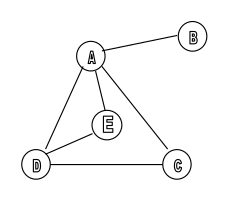
\includegraphics[scale=0.60]{neor_graf.png}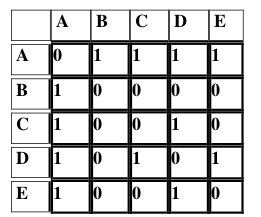
\includegraphics[scale=0.58]{matrix_n_graf.png}
  \caption{Príklad neorientovaného grafu a jeho matice}
  \label{fig:graf}
\end{figure}

\textbf{Implementácia} neorientovaného grafu je pomocou matice koincidencie t.j spojenia. Táto matica je symetrická podľa hlavniej diagonály.

\textbf{Zafarbením grafu} rozumieme priradenie farieb uzlom grafu, pričom žiadne dve susedné uzly nesmú byť zafarbené rovnako. Minimálny počet použitých farieb se nazýva \textbf{chromatické číslo}. Práve toto chromatické číslo v našom projekte hľadáme. 

[\textcolor{red}{EDIT: }Právě řešení s tímto chromatickým číslem v našem projektě hledáme.]

\subsection{Popis projektu}
\textbf{Spúštanie:} ./main -f FILENAME [-h] [-b], kde
\begin{itemize}
    \item -f FILENAME je názov súboru, ktorý obsahuje maticu grafu
    \item -b je volitelný parameter, ktorý má na starosti...
    \item -h je volitelný parameter, ktorý má na starosti vytlačiť spravu pre používanie na stdout
\end{itemize}

\section{Testování projektu}
Projekt sme najskôr testovani na menšich testovacích grafoch, ktoré sme vytvorili a vedeli aj odkontrolovať. Neskôr sme na generovanie grafov vytvorili skript, ktory vytvoril aj väčšie grafy. Testovanie prebiehalo na platforme Ubuntu, MacOS a FreeBSD.

\section{Implementácia}
[\textcolor{red}{TRANSLATE: }Všechno pod tímto přeložit]
\subsection{Struktury}
\subsection{Algoritmus}
\subsection{Analýza složitosti algoritmu}

\section{Záver}
TBD

\section{Zdroje}
opora ial,
izu prednasky,
prednasky ial, 

\end{document}